
\section{Dataset}
\label{section: setup baseline dataset - dataset}

%       -------------------------------
%     [[ Frame-by-frame data structure ]]
%       -------------------------------
% Explain the division between "initialization frames" and "usage frames", why this is important, and how this specification is made (timestamp at MEB initialization).
% Explain the different characteristics of these two types of frame data (initialization has both hands at the same time)
% Mention that this "initialization" is on a \textit{recording-by-recordings} basis
% Refer to the frame count appendix

In order to properly compare IAmMuse to the state-of-the-art solutions, we'll need a clear specification of the data that is available.
First, a distinction will be made between two types of frames within any singular recording of the system.
During the usage of the system, users were first instructed to initialize the system, as is specified in \cref{sub-section: tracking method - data enhancement - minimal enclosing ball}.
Only after this initialization could the users actually use the system, since this initialization was required in order to do the data interpretation. 
Due to this, there are two distinct parts of each recording, where the user acts very differently in each, a visualization of which is visible in \cref{fig:frame_types}.
Firstly, we have the \textbf{initialization data}, the data prior to the user being told that the initialization is complete, where the user moved both hands up and down at a steady pace.
Secondly, we have the \textbf{usage data}, from the moment the user was told that the system was initialized. 
In this data, the user will move their hands to specific zones and hold them there for an amount of time to generate a note.
It's important to make a distinction between these two types of data since the user behavior is inherently different in both these systems, but also because IAmMuse (by definition) only evaluates the \textit{usage data}, thus any comparison between IAmMuse and a different system must be a comparison over the results when applied to the \textit{usage data}.
The separation between \textit{initialization data} and \textit{usage data} is the moment when the initialization has completed.
The exact number of frames of \textit{initialization data} and \textit{usage data} for each recording can be found in Appendix \ref{appendix: recording frame distribution}.

\begin{figure}[h]
    \centering
    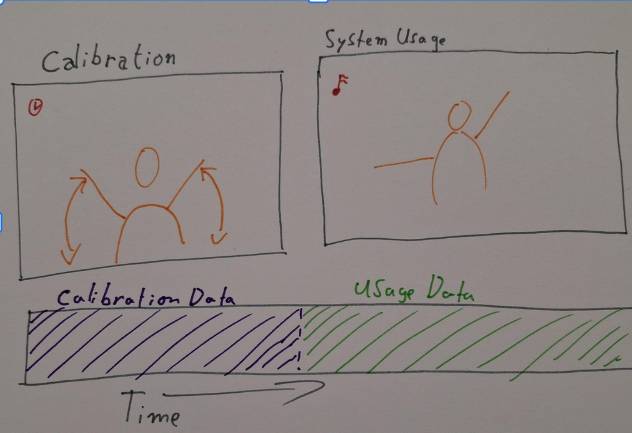
\includegraphics[width=0.7\linewidth]{figures/experimental setup/frame_types.png}
    \caption{Visualization of the two frametypes present in each recording}
    \label{fig:frame_types}
\end{figure}




%         ---------------------------
%       [[ Different recording types ]]
%         ---------------------------
Describe the two types of recordings which exist, \textbf{standard} and \textbf{free play}.
Specify that this is \textbf{only} applicable to the \textit{usage frames} and that the type of initialization is the same.
Explain why this choice for standardized was made (comparability over recordings)
Explain why the choice for free play was made (more realistic system usage data)
Refer to the standardized movement set appendix

%         -----------------
%       [[ Different users ]]
%         -----------------
Discuss the different users, the number we had, and the variations in them.
Specify that \textit{a few recordings} got \textbf{corrupted} (failed to save, for one reason or another)
Specify that different users made a different number of \textit{free play} recordings

%         -----------------------
%       [[ Recap and terminology ]]
%         -----------------------
Small recap, quickly describing the different terms used, such as the \textit{types of frames}, \textit{types of recording}, etc

% Explain what data was collected, 

% define some common terms used throughout other parts of the dataset and evaluation parts (two types of recordings, initialization data, evaluation data, etc.)

